\section{En trigonometría}

\label{1:sec:1}
En trigonometría el seno de un ángulo en un triángulo rectángulo se define como la razón entre
el cateto opuesto y la hipotenusa:\[f(x)=sin(x)\]
O también como la ordenada correspondiente a un punto que pertenece a una circunferencia unitaria
centrada en el origen (c=1):\[sin \alpha =a\]
En matemáticas el seno es la función continua y periódica obtenida al hacer variar la razón mencionada,
siendo una de las funciones trascendentes.
\begin{figure}[H]
\begin{center}
\includegraphics[scale=0.2]{images/seno.eps}
\end{center}
\caption{FuncionSeno}
\label{graph:3}
\end{figure}

\section{El seno en programación}
\label{1:sec:2}

   Antes de comenzar, se debe destacar  que de forma habitual, todos los
lenguajes de programación proveen una función seno, así como el resto de 
funciones trigonometrícas. También es normal  que el ángulo que recibe la
función deba pasarse en radianes.

  Esto último es importante tenerlo en cuenta ya que podrían derivarse errores
por este concepto. Del mismo modo las calculadoras suelen aceptar el valor 
en grados o radianes, siendo necesario para realizar el cálculo correctamente
activar un botón selector del tipo de grados que se desea usar.

  A continuación se muestra un ejemplo, obsérvese como la escasa diferencia entre
ambos valores resultantes podría pasar desapercibida. Por ello, cuando sea conveniente
se recomienda pasar los grados a radianes o viceversa.
\begin{figure}[h]
\begin{center}
\includegraphics[scale=0.5]{images/ejemplo_seno.eps}
\end{center}
\caption{EjemploSeno}
\label{graph:5}
\end{figure}
